\documentclass[main.tex]{subfiles}
\begin{document}
\chapter{Conclusion and Future Work}
\label{chap:concl}

% \paragraph{intro summary}
Modern man-made environments, especially indoors, contain a large number of planar structures. The automatic detection thereof has become a vital part of many Augmented or Virtual Reality systems. Underlying temporal constraints often dictate the processing times of these applications and, therein, the process of plane detection. Real-time plane detection is already possible, although the hardware cost that enables efficient and precise detection is likely not affordable to the general consumer.
Therefore, the extent of \textit{real-time} plane detection on affordable hardware has gained interest.

% \paragraph{concept summary}
A set of plane detection algorithms, appropriate datasets, and a definition of \textit{real-time} are needed to perform this evaluation. In the \textit{Concept}, we first introduced a set of helpful criteria for the subsequent selection of plane detection algorithms. We followed the same approach for the selection of datasets. Lastly, we introduced two definitions of \textit{real-time}, wherein we differentiate between \textit{real-time} calculation time with and without pre-processing.

% \paragraph{impl summary}
In Chapter~\ref{chap:impl}, we provided details regarding the implementation of the selected algorithms. Moreover, since its provided ground truth does not focus on planes, we described our manual segmentation process of the 2D-3D-S dataset. Lastly, we outlined how the ground truth for the FIN dataset is dynamically created based on a single ground truth of the last recorded point cloud.
% \paragraph{eval summary}
We enter Chapter~\ref{chap:eval} with the evaluation protocol. Therein, we outline the evaluation metrics to calculate and specify the algorithm parameterizations of each experiment. We presented the individual results and subsequently concluded with a comparison thereof.

% accuracy
In both experiments, RSPD has the overall best accuracy among the algorithms. While OPS and OBRG achieve a similar average \textit{Precision}, no other algorithm yields comparable values for \textit{Recall} nor \textit{F1-Score} (see Tables~\ref{tab:res-3d2ds-total} and \ref{tab:res-fin-total}). The accuracy metrics of all algorithms drop by roughly $30\%$ from the \textit{2D-3D-S} experiment to the \textit{FIN} experiment.

% times
The results uniformly show that 3D-KHT is the fastest among the selected algorithms. The \textit{Hough Transform}-based algorithm proposed by \citeauthor{LimbergerOliveira2015HT3D}~\cite{LimbergerOliveira2015HT3D} ran, on average, 32x faster than the other algorithms. As Table~\ref{tab:algo-rt} indicates, 3D-KHT is the only algorithm that achieves $RT_{tot}$ in the \textit{FIN} experiment, which is supported by the apparent upper limit shown in Figure~\ref{fig:dynaudi}. RSPD achieves $RT_{calc}$, and OPS borders on \textit{Real-Time Plane Detection}applicability as well. RSPD has the longest pre-processing times with an average of ${\sim}63s$ for the \textit{2D-3D-S} experiment and ${\sim}15s$ for the \textit{FIN} experiment, respectively. In contrast, RSPD has the shortest average plane detection times in the \textit{FIN} experiment, and takes only a tenth of a second longer than 3D-KHT's plane detection phase in the \textit{2D-3D-S} experiment.

% Summary 
We can conclude that 3D-KHT is the only algorithm that achieves \textit{Total Real-Time} applicability. However, considering accuracy, 3D-KHT is inferior to RSPD.


\section{Limitations}
This section deals with the limitations of the concept, evaluation, and results thereof.
\paragraph{Algorithm Parameterization}
Since the focus of this work is not the optimization of plane detection algorithms but rather the evaluation thereof, the parameterizations used during the experiments are likely non-optimal. Furthermore, the required effort would go beyond the scope of this work. Integrating a plane detection algorithm into an application would require extensive parameter optimization w.r.t. the expected environment, the used sensors, and the general use case.

\paragraph{Manual Segmentation}
Another limitation of the results is the subjective nature of the manual segmentation process described in Section~\ref{sec:gtseg}, which influences the evaluation. The effect thereof does not seem significant for the \textit{2D-3D-S} experiment. However, the segmentation can lead to errors due to the level of noise in the \textit{FIN} dataset. For instance, with increasing "thickness" of planes, the number of possible orientations of a detected plane also increases (see Figure~\ref{fig:poss-planes}). The red segment in the figure represents the ground truth we selected to represent the plane. If an algorithm detected a plane in one of the four other variants, both the voxel overlap and the accuracy would decrease, even if both planes correspond.

\begin{figure}
    \centering
    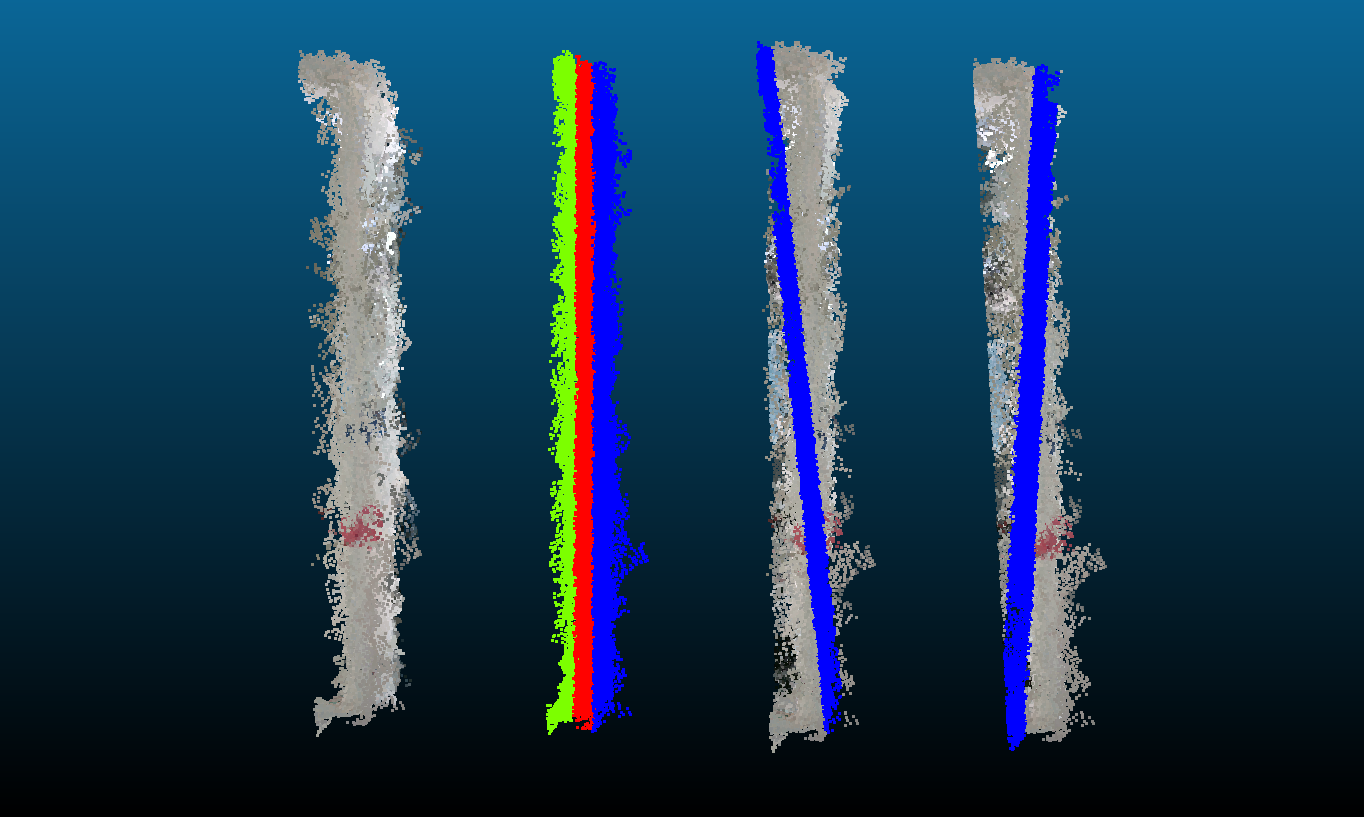
\includegraphics[width=0.7\textwidth]{images/possible_planes.png}
    \caption[Plane Orientation Ambiguity]{Possible Plane Orientations. Shown is the top view of a wall with a width of ${\sim}1$m from the \textit{conference room} scene of the \textit{FIN} dataset is shown on the left. The colored point clouds indicate different possible plane orientations.}
    \label{fig:poss-planes}
\end{figure}

\paragraph{Used Technology}
A small caveat to note is that the FIN dataset is recorded using a specific combination of technology, namely Intel's T265, D455, and the corresponding SDK including RTAB-MAP.
Since these sensors were chosen as representatives for consumer off-the-shelf hardware, the results point out the general applicability in a realistic environment. However, the results may vary when employing different technology. 

\section{Future Work}
\paragraph{Normal Estimation}
We see the most potential for improvement in the pre-processing steps of the algorithms. Specifically, the extent of the normal vector estimation influences the pre-processing time. RSPD estimates the normal vectors of the entire point cloud, whereas OPS only estimates a certain percentage of the point cloud. This temporal difference raises the question of what the extents of \textit{real-time} plane detection are if the normal vectors of the point cloud are known before the plane detection step in the application. For instance, RTAB-MAP can estimate and export the normal vectors of the point cloud. Therefore, RSPD would not need to estimate the normal vectors, reducing the pre-processing time greatly. However, this would require further research.

\paragraph{Cloud Size Reduction}
When recording environments similar to the hallway or the auditorium scene, it is often the case that the spatial dimension of the point cloud grows beyond the distance limitations of the sensor, e.g., the recorded hallway spans longer than the sensor can "see". It is, therefore, not necessary to re-calculate the planes in areas past the sensor's reach. We are interested in a plane detection method that restricts the plane detection to a certain radius around the sensor's position and a subsequent merging of old and new planes. Additionally, this could be the basis for a plane-based SLAM approach.

\paragraph{Outdoor Environment}
In Chapter~\ref{chap:Introduction}, we limited ourselves to evaluating plane detection algorithms in indoor environments. Therefore, we cannot make any statements about the applicability in outdoor environments. Since we compiled results in a realistic indoor environment, it would be interesting to evaluate the generalization of these algorithms. As discussed throughout this thesis, a comparison needs uniformity. Since we created an indoor dataset, selected datasets, and provided all necessary metrics and definitions, only an appropriate dataset is needed.

\end{document}